\documentclass[
  % all of the below options are optional and can be left out
  % course name (default: 2IL50 Data Structures)
  course = {{DS12E Clustering Algorithms}},
  % quartile (default: 3)
  quartile = {{2}},
  % assignment number/name (default: 1)
  assignment = ,
  % student name (default: Some One)
  name = {{Michael Darmanis ; Vasilios Venieris}},
  % student number, NOT S-number (default: 0123456)
  studentnumber = {{7115152200004 ; 7115152200017}},
  % student email (default: s.one@student.tue.nl)
  email = {{mdarm@di.uoa.gr ; vvenieris@di.uoa.gr}},
  % first exercise number (default: 1)
  firstexercise = 1
]{aga-homework}

\begin{document}

\section{Introduction}

This project uses the data provided in the file \texttt{Salinas\char`_Data.mat}, which contains a $150x150x204$ three-dimensional matrix named \texttt{Salinas\char`_Image} (representing the Salinas hypercube) and a $150x150$ two-dimensional image named \texttt{Salinas\char`_Labels} (representing the class label for each pixel). The aim of this project is to compare the performance of different clustering algorithms in finding homogeneous regions within the Salinas HSI.

The objective is to compare the performance of cost function optimisation clustering algorithms (e.g. k-means, fuzzy c-means, possibilistic c-means and probabilistic clustering) and hierarchical algorithms (e.g. complete-link, WPGMC and Ward algorithms) in identifying homogeneous regions within the Salinas hyperspectral image. The analysis will be restricted to those pixels for which class label information is available.

To achieve this goal, the following tasks will be executed:
\begin{itemize}
\item Execution of all above algorithms, for various combinations of their parameters (e.g. the number of clusters etc.) in order to identify the homogeneous regions in the image, and reporting any encountered problems.
\item Qualitative verification of the results obtained by each algorithm in terms of (i) the pixel label-information and (ii) information that can be gathered by the image (.i.e examining principal components).
\item Quantitative verification of the results in terms of the labelling information.
\item Comparison of the overall clustering accuracy for each algorithm.
\end{itemize}

The aim of the project is to gain insight into how different clustering algorithms perform on the Salinas HSI and to identify which algorithm is best suited to this type of data. Although not explicitly stated, extensive use was made of the following textbooks Pattern Recognition\cite{pattern} and Mining Massive Datasets\cite{leskovec}.

\section{Methodology}

Before clustering algorithms are applied, a two-step process is used in which: (i) the dimensionality of the data is reduced, and then (i) k-means clustering is performed in the low-dimensional feature space to determine the optimal number of clusters. PCA followed by k-means performs linear dimensionality reduction on the input image to be clustered.

\subsection{Hyperspectral dataset}

More specifically, after loading the data, each feature of the dataset is normalised with respect to its mean and its range. Principal component analysis (PCA) is then applied to the normalised data to determine the optimal number of components to retain, while still retaining at least $99\%$ of the variance in the data set. However, variance explainability does not necessarily imply reconstructability. This is clearly shown in the \texttt{biplot} \cite{biplot} of Figure~\ref{fig:bplot}.

\begin{figure}[htbp!]
  \centering
  \def\svgwidth{.7\linewidth}
  \input{figures/plot1.pdf_tex}
  \caption{Principal components retaining 99\% of the initial variance.}
  \label{fig:bplot}
\end{figure}

While the two principal components retain more than $99\%$ of the data (red dots), the vectors (blue line segments) have a large angle, indicating a loss in reconstruction. However, this worst case is a necessity. Due to the high dimensionality of the data (204 bands), PCA is performed for reasons of computational efficiency, while allowing a more heuristic and less rigorous analysis.

The Calinski-Harabasz criterion and the "elbow" method are then used to determine the optimal number of clusters, as can be seen in Figure~\ref{fig:k-init}. The optimal number of clusters was found to be

\begin{verbatim}
Enter the number of clusters k (Calinski-Harabasz criterion = 7, Elbow Method = 5):
\end{verbatim} 

It should be noted that the ``elbow'' method is a heuristic method used to determine the number of clusters, by fitting the model with a range of number of clusters and looking for an ``elbow'' point on the within-cluster sum of squares (WCSS) plot, where the increase in WCSS slows down. The fallacious indication of 5 number of clusters is a result of an attempted automation of the process using the second derivative as can be seen in the following part of the code:

\begin{verbatim}
% Calculate the second derivative of the WCSS
d2 = diff(diff(wcss));

% Find the local maxima of the second derivative
[~, idx] = findpeaks(-d2);

% The optimal number of clusters is the number of clusters where the second
% derivative changes sign
k1 = idx(1) + 2;
\end{verbatim}

\begin{figure}[htbp!]
\centering
\begin{subfigure}{0.45\textwidth}
    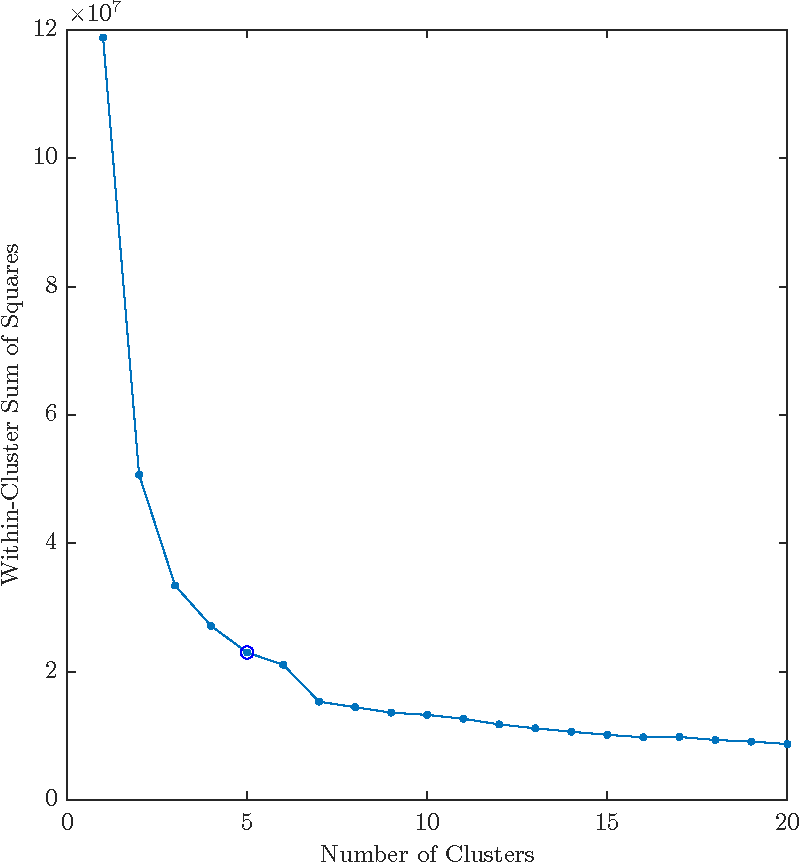
\includegraphics[width=\textwidth]{elbow}
    \caption{``Elbow'' method.}
    \label{fig:elbow}
\end{subfigure}
\hfill
\begin{subfigure}{0.45\textwidth}
    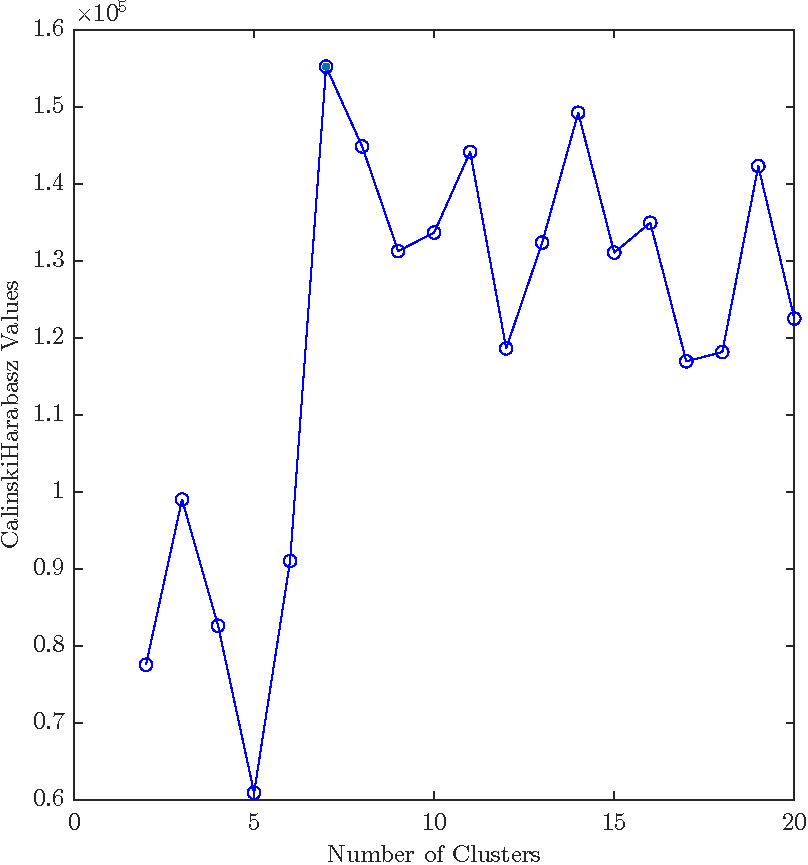
\includegraphics[width=\textwidth]{eval}
    \caption{Variance-ratio criterion.}
    \label{fig:eval}
\end{subfigure}
        
\caption{Picking the right number of initial clusters k.}
\label{fig:k-init}
\end{figure}

The analysis will thus proceed with 7 number of clusters.

\subsection{Implementation}

After pre-processing and dimensionality reduction, the modified data is then subjected to a comprehensive examination using a variety of clustering algorithms. These algorithms include both cost function optimisation techniques and hierarchical approaches. Specifically, the cost function optimisation algorithms used in this analysis include k-means, fuzzy c-means, possibilistic c-means and the probabilistic algorithm. Hierarchical algorithms such as complete linkage, weighted pair group method with arithmetic mean (WPGMA) and ward linkage are also used.

The hierarchical algorithms are applied to the same dataset as the cost function optimisation algorithms and the results obtained are compared with those obtained using the original label figure. The subsequent analysis is both qualitative and quantitative, with particular emphasis on assessing the overall clustering accuracy of the algorithms employed.

\section{Experiments and results}

Most of the clustering algorithms used in this analysis are run while varying a number of their parameters. The optimal run, determined by a specific criterion, is then retained for comparison. The reconstructed images based on the clustered labels are presented using principal component analysis. In the case of hierarchical algorithms, dendrograms are also presented for clarity. Finally, the best results of each algorithm are evaluated using the Adjusted Rank Index (ARI) \cite{ard} and the Normalised Mutual Information (NMI) \cite{nmi} as performance metrics.

\subsection{Cost-function-optimisation algorithms}

The k-means algorithm is used first, where it is run multiple times to select the iteration with the lowest sum of distances (sumd) between the data points and their corresponding cluster centroids. It was found that a modification of the metric distance was necessary due to the presence of noise in the data, so its variant (the k-medians) was actually executed. The resulting cluster assignments are then used to assign class labels to each pixel.

The fuzzy c-means algorithm is then used, with different values for the fuzzifier parameter, and the iteration with the lowest cost function value is selected. The resulting cluster assignments are then used to assign class labels to each pixel.

The Possibilistic c-means algorithm is then used with a fixed eta, a q-number of 40 and a random initialisation of centroids to assign class labels to each pixel. No attempt was made to automate the process. Parameter variation was done manually and the best quantitative result was kept.

Finally, a probabilistic algorithm is used to fit a Gaussian mixture model to the data for different values of k, considering two types of covariance (a full covariance matrix and a diagonal). The model with the lowest Bayesian Information Criterion (BIC) \cite{bic} value is selected and the resulting cluster assignments are used to assign class labels to each pixel.

\begin{figure}[htbp!]
	\centering
    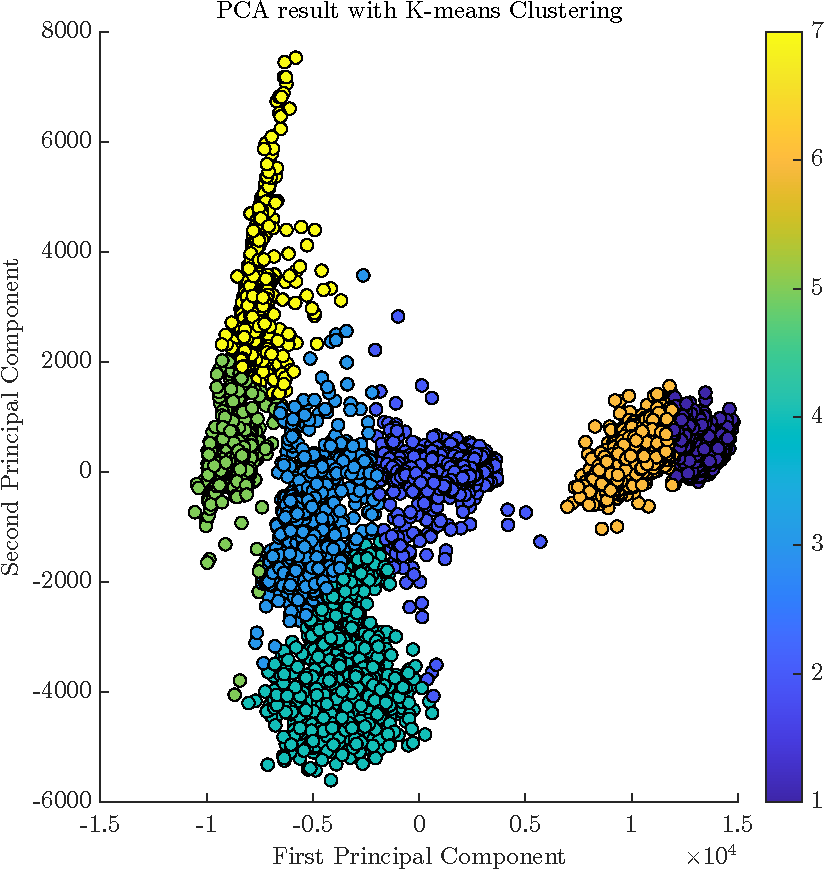
\includegraphics[scale = 0.6]{pca-k-means}
    \caption{Principal components on the resulting k-means clustering.}
    \label{fig:k-means}
\end{figure}

\begin{figure}[htbp!]
	\centering
    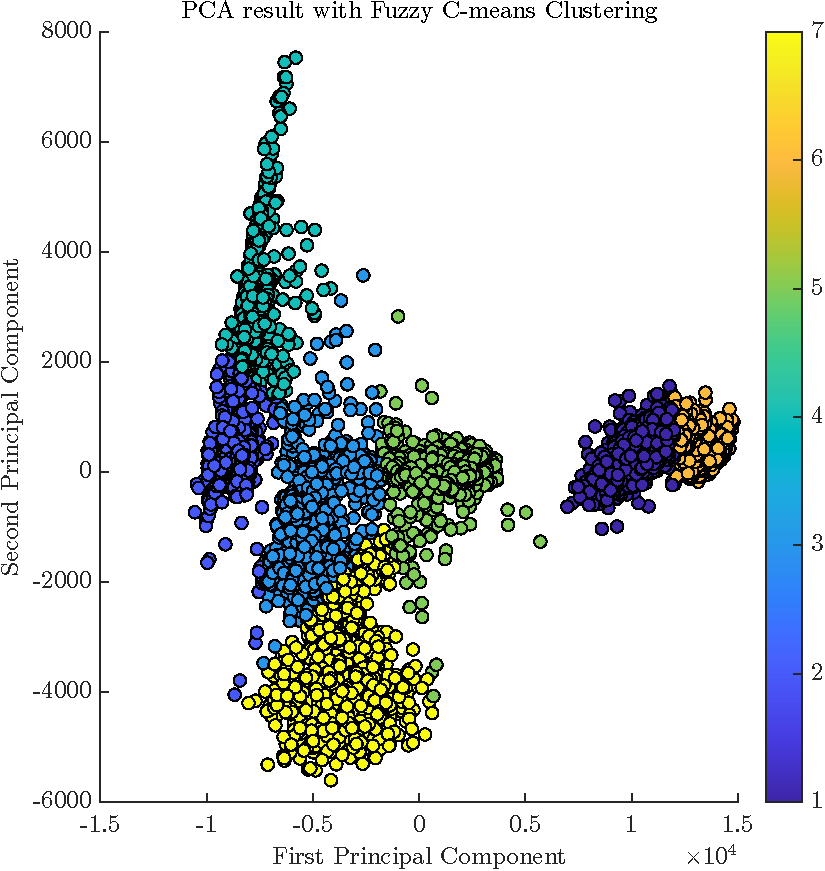
\includegraphics[scale = 0.6]{pca-fuzzy}
    \caption{Principal components on the resulting fuzzy c-means clustering.}
    \label{fig:fuzzy}
\end{figure}

\begin{figure}[htbp!]
	\centering
    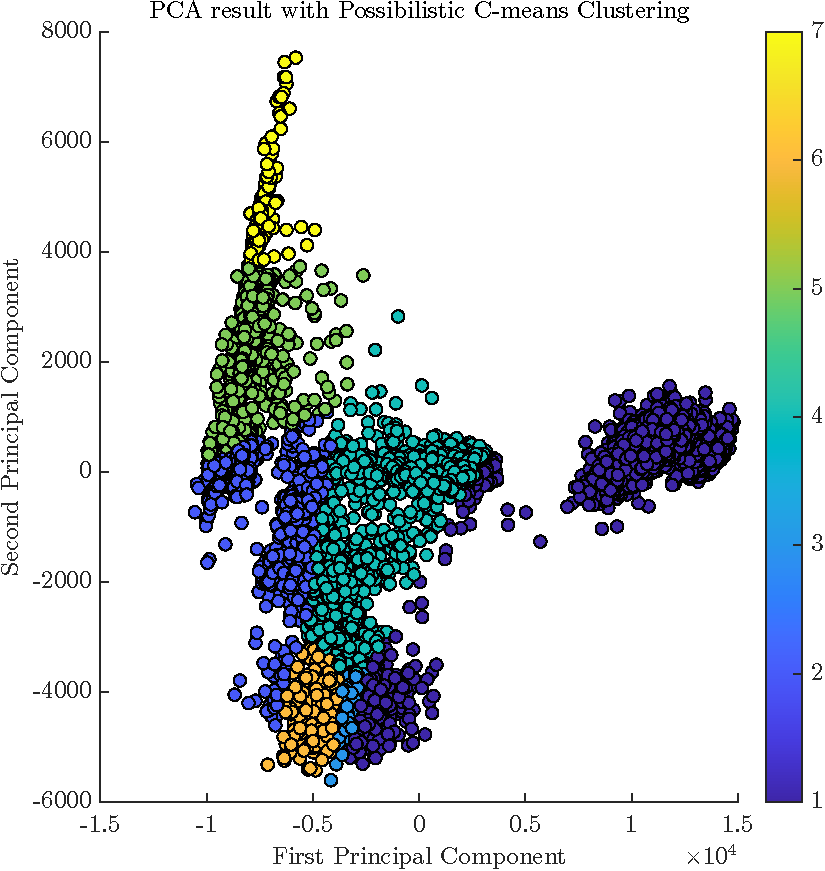
\includegraphics[scale = 0.6]{pca-possibi}
    \caption{Principal components on the resulting possibilistic c-means clustering.}
    \label{fig:possibi}
\end{figure}

\begin{figure}[htbp!]
	\centering
    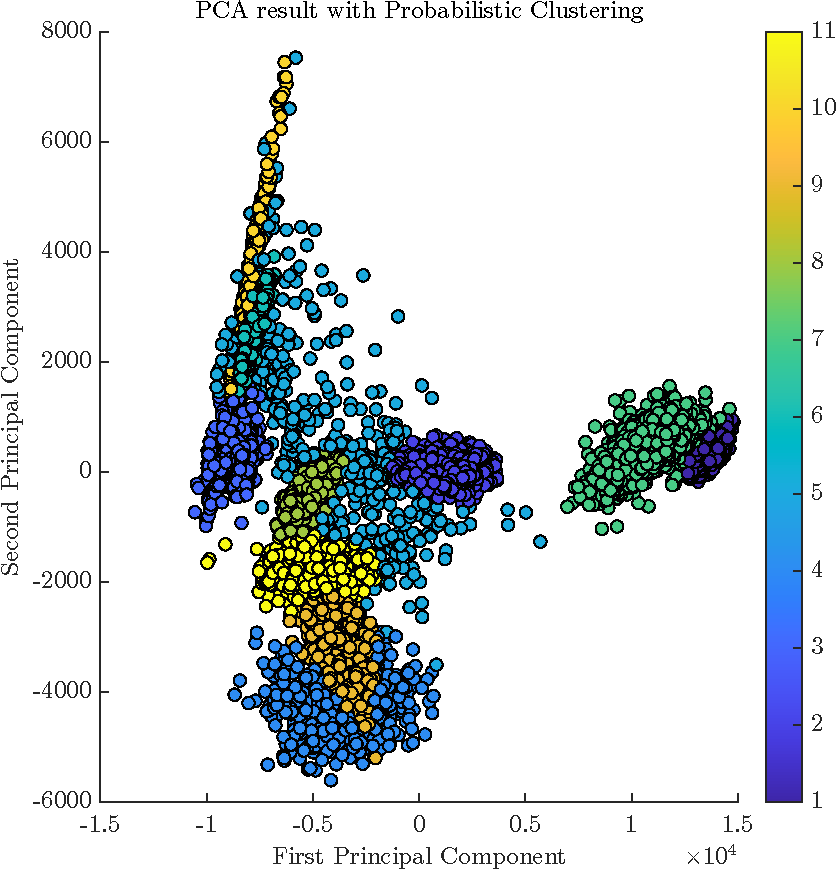
\includegraphics[scale = 0.6]{pca-probabi}
    \caption{Principal components on the resulting probabilistic clustering.}
    \label{fig:probabi}
\end{figure}


\FloatBarrier
\subsection{Hierarchical algorithms}

Three hierarchical clustering algorithms were applied to the modified data obtained from pre-processing and dimensionality reduction. The complete linkage, weighted pair group method with arithmetic mean (WPGMC) linkage, and Ward linkage algorithms were employed.

The complete linkage algorithm was applied by first computing the pairwise distances between the data points using a pool of dissimilarity metrics, including Euclidean, cityblock (Manhattan), Mahalanobis, and Chebychev. The linkage algorithm was then applied to the resulting distance matrix. The script then calculated the cophenetic correlation coefficient between the resulting linkage matrix and the original distance matrix, and selected the linkage matrix and the corresponding metric that resulted in the highest coefficient. The best linkage matrix and the corresponding metric were then used to assign class labels to each pixel. The distance yielding the best results was the Manhattan one, as the script's output indicates:

\begin{verbatim}
The best metric, for complete linkage, is cityblock with a cophenetic correlation
coefficient of 0.904063
\end{verbatim}

The WPGMC linkage and Ward linkage algorithms were also applied, using only the Euclidean distance to compute pairwise distances. The linkage matrices obtained in this step were visualised using dendrograms to provide further clarification.

It is worth noting that the complete-linkage algorithm permits the use of any proximity measures, and results will depend on the chosen measure. However, for the WPGMC and Ward linkage algorithms, only squared Euclidean distances should be used for the sake of geometric correctness, as these methods compute centroids in Euclidean space.

The termination criterion for all of the above-mentioned algorithms was the initially calculated ideal number of clusters, which was set to 7.


\begin{figure}[htbp!]
	\centering
    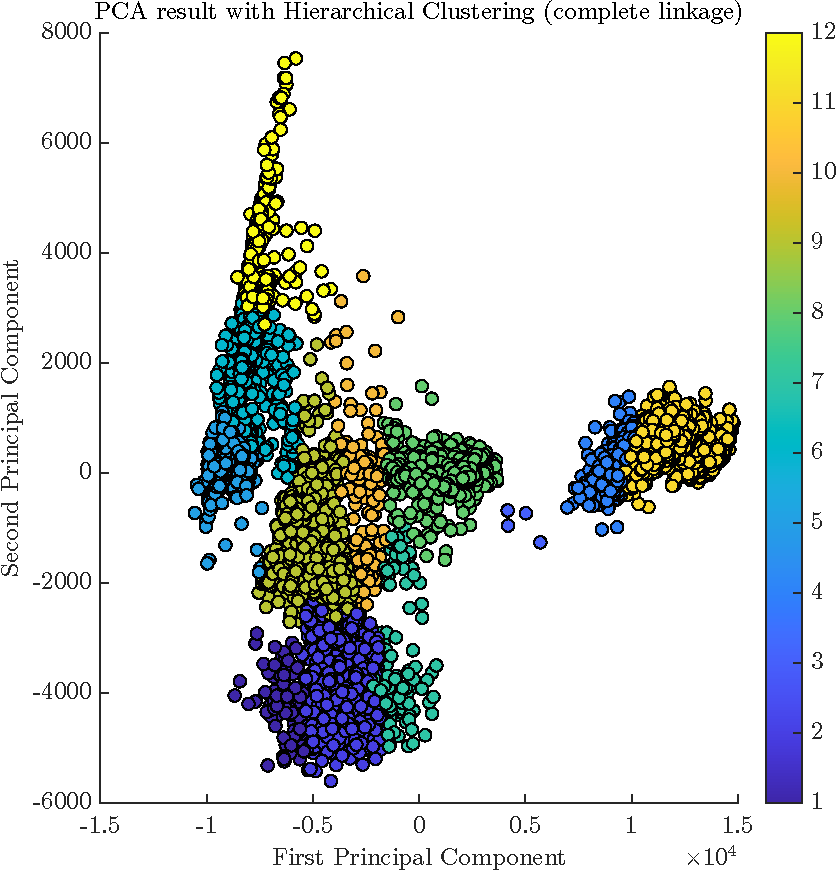
\includegraphics[scale = 0.6]{pca-h-c}
    \caption{Principal components on the resulting hierarchical clustering with complete linkage.}
    \label{fig:h-complete}
\end{figure}

\begin{figure}[htbp!]
  \centering
  \def\svgwidth{.7\linewidth}
  \input{figures/complete-link.pdf_tex}
  \caption{Dendrogram of hierarchical algorithm with complete linkage.}
  \label{fig:h-complete-dendo}
\end{figure}

\begin{figure}[htbp!]
	\centering
    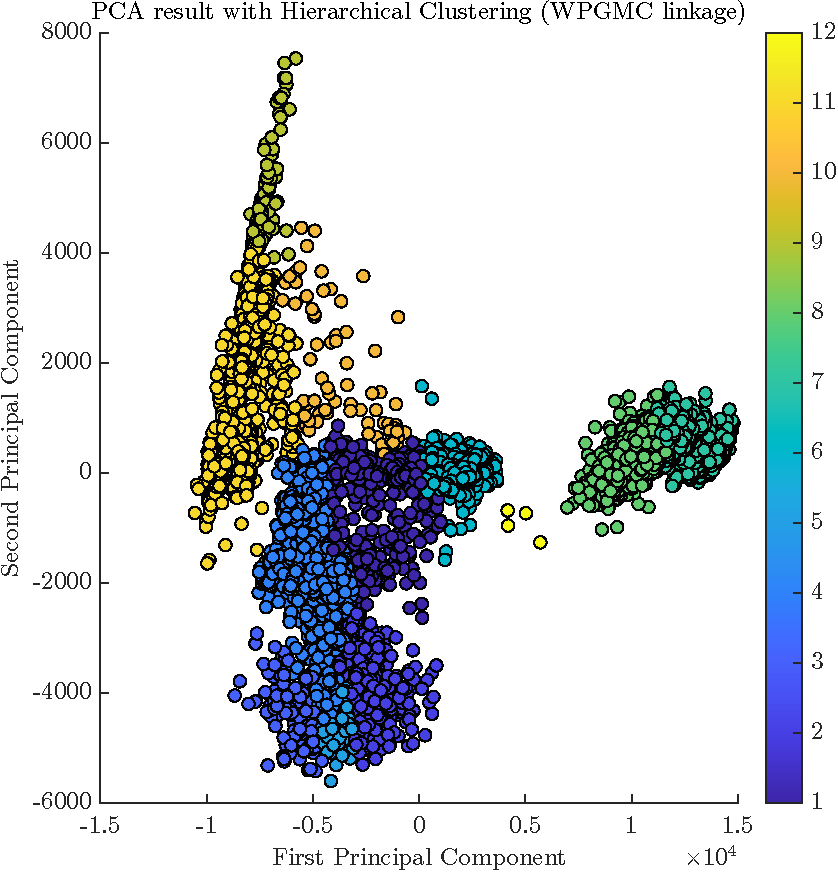
\includegraphics[scale = 0.6]{pca-h-wpgmc}
    \caption{Principal components on the resulting hierarchical clustering with WPGMC.}
    \label{fig:h-wpgmc}
\end{figure}

\begin{figure}[htbp!]
  \centering
  \def\svgwidth{.7\linewidth}
  \input{figures/WPGMC.pdf_tex}
  \caption{Dendrogram of hierarchical algorithm with WPGMC.}
  \label{fig:h-wpgmc-dendo}
\end{figure}

\begin{figure}[htbp!]
	\centering
    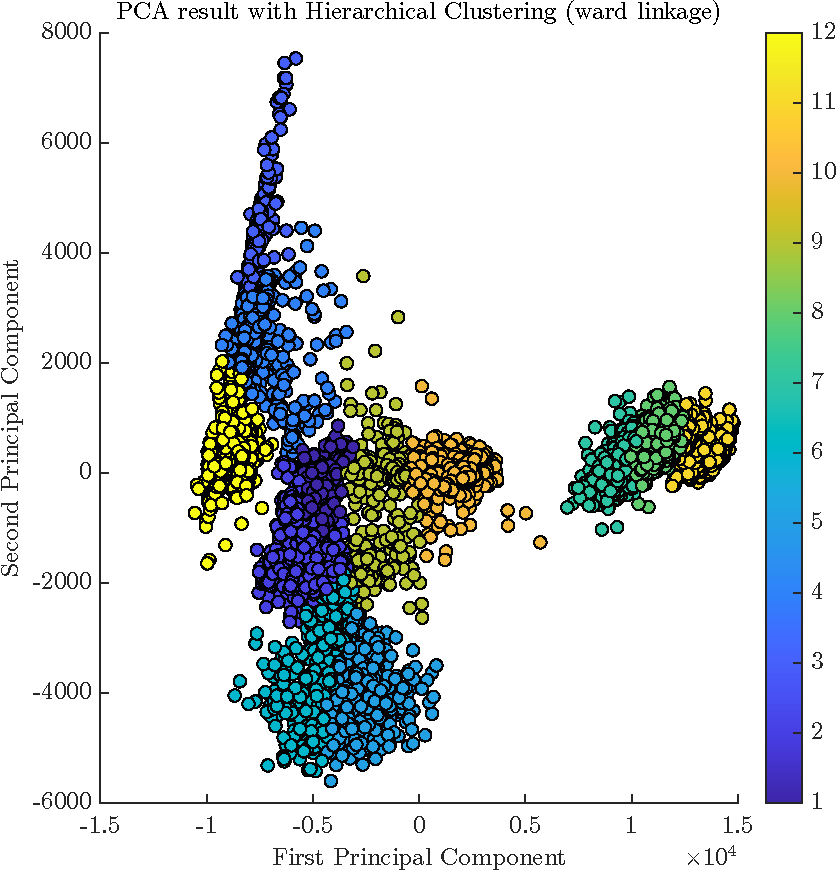
\includegraphics[scale = 0.6]{pca-h-ward}
    \caption{Principal components on the resulting hierarchical clustering with Ward.}
    \label{fig:h-ward}
\end{figure}

\begin{figure}[htbp!]
  \centering
  \def\svgwidth{.7\linewidth}
  \input{figures/ward.pdf_tex}
  \caption{Dendrogram of hierarchical with Ward.}
  \label{fig:h-ward-dendo}
\end{figure}

\FloatBarrier
\subsection{Qualitative evaluation}

Figure~\ref{fig:reconstructed} showcases the reconstructed figure using the clustered labels, while Figure~\ref{fig:original} is a representation of the two principal components of the original figure.

\begin{figure}[htbp!]
	\centering
    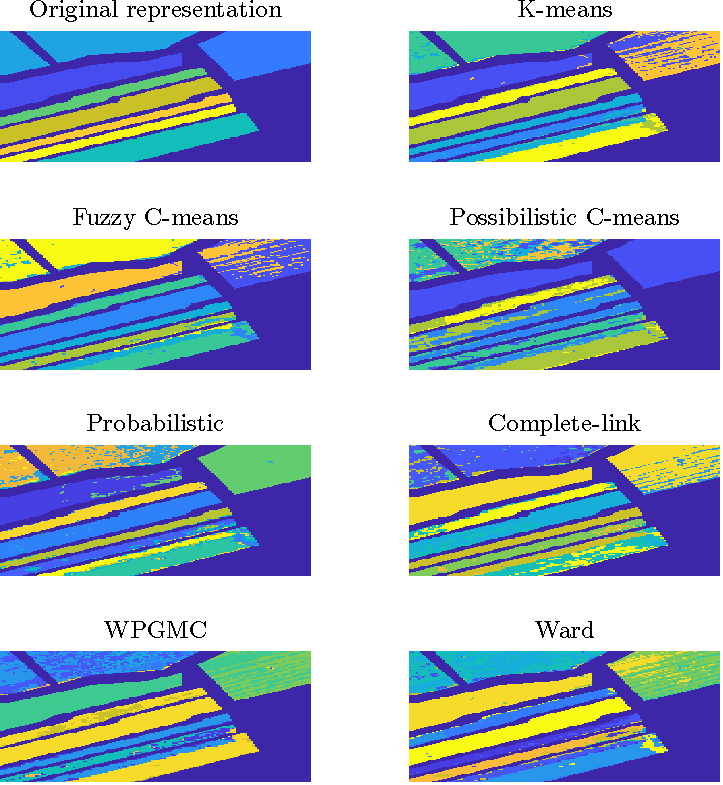
\includegraphics[scale=0.8]{reconstructed}
    \caption{Reconstructed images, using original labels and resultant clustering labels.}
    \label{fig:reconstructed}
\end{figure}

\begin{figure}[htbp!]
	\centering
    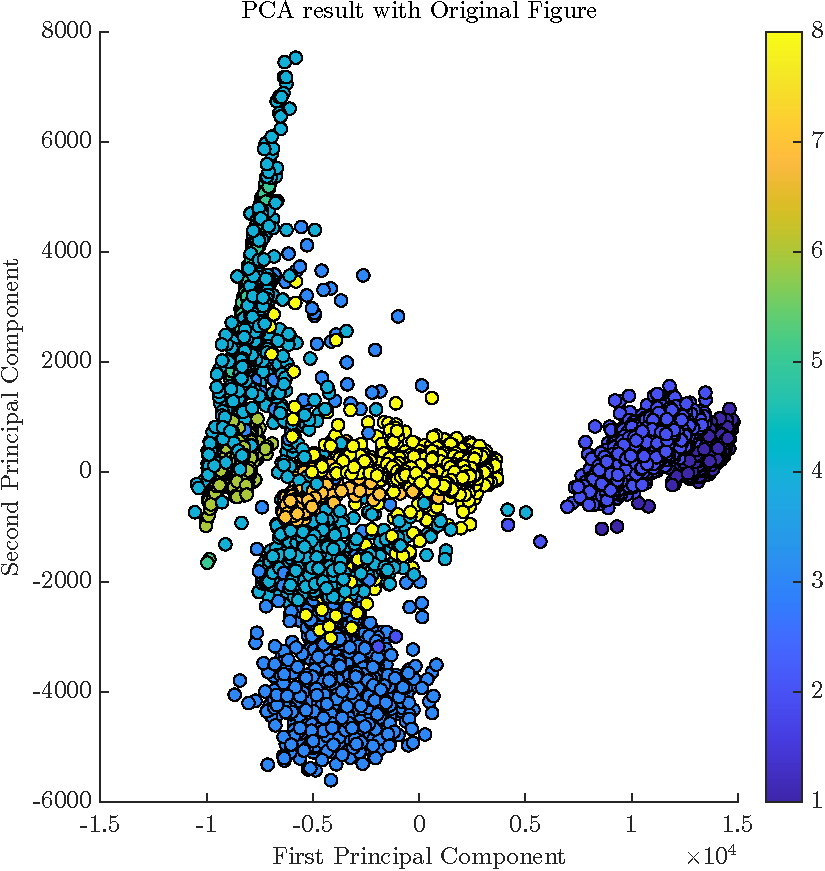
\includegraphics[scale = 0.6]{pca-original}
    \caption{Principal components of the original representation.}
    \label{fig:original}
\end{figure}

The k-means and fuzzy c-means algorithms were found to produce similar results in identifying the underlying structure of a dataset, as shown in Figures~\ref{fig:k-means} and \ref{fig:fuzzy}. The fuzzy c-means algorithm is an extension of the k-means algorithm that allows for overlapping clusters, but this feature did not prove beneficial in the case study. A limitation of both algorithms is that they assume compact clusters with equal variances and are sensitive to noise. While applying the algorithms several times with different initial conditions can mitigate the first drawback, the issue of cluster shape remains unresolved.

The possibilistic c-means algorithm, another extension of the k-means algorithm, allows for overlapping clusters. However, it has been found to produce the worst clustering results among the cost function optimisation algorithms, as shown in Figure~\ref{fig:possibi}. This is mainly due to the lack of proper parameterisation and the influence of noise on its efficiency. Theoretically, the probabilistic c-means algorithm could be ideal for the Salinas dataset if properly parameterised.

In contrast, the probabilistic clustering algorithm is based on the assumption that the data follows a Gaussian mixture model. Like the previous algorithms, it is sensitive to initial conditions. This algorithm produced the best result when assuming a diagonal covariance matrix for the clusters, as shown in Figure~\ref{fig:probabi}. It was able to capture the nuanced structure of the Salinas dataset. However, it should be noted that the best result corresponded to 11 clusters, which were found to be incorrect by external validation, as shown in Figure~\ref{fig:original}.

The complete linkage method, as shown in Figure~\ref{fig:h-complete}, does reveal some clusters, but they are not homogeneous. This is due to the method's metaphor of cluster formation, which is similar to a circle in which the two most distant members cannot be much more dissimilar than other dissimilar pairs. Such clusters are compact at their boundaries, but not necessarily compact inside, and are sensitive to noise.

The WPGMC algorithm also performs poorly at identifying compact clusters, as shown in Figure~\ref{fig:h-wpgmc}. This is due to the fact that the cluster centroids are defined such that the sub-clusters have an equal influence on their centroid, regardless of the number of objects in each sub-cluster. This method is also sensitive to the initial configuration of the data and is not well suited to dealing with clusters of different sizes or shapes, as it tends to produce clusters of similar size and shape. In addition, its implementation in this case did not converge to a global optimum due to an instance of non-monotonicity.

Finally, Ward's method, as seen in Figures~\ref{fig:h-ward} and \ref{fig:k-means}, is the closest to k-means clustering in terms of properties and efficiency. Both methods have the same objective function, which is to minimise the sum of squares pooled within the cluster. While k-means, given appropriate initial centroids, is a better minimiser of this function, Ward's method has been found to be more accurate in detecting clusters of uneven physical size or clusters that are irregularly distributed in space.

\subsubsection{Hierarchical algorithms' miscluster}

In the present study, a cut-off of seven clusters was specified for the implementation of all hierarchical clustering algorithms. However, it was observed that all algorithms returned twelve clusters instead.

One possible explanation for this discrepancy may be that the cut-off of seven clusters was not appropriate for the data and the specific hierarchical algorithms employed. The determination of the number of clusters is often based on domain knowledge or heuristics, however, it may also be estimated through the utilization of methods such as the elbow method or the silhouette score. Thus, it is plausible that the chosen cut-off of seven clusters did not accurately reflect the true underlying structure of the data.

Another potential explanation for this discrepancy is that the hierarchical algorithms utilized in this project tend to favour larger numbers of clusters and may not have been able to effectively identify the desired number of clusters. Hierarchical algorithms typically rely on linkage criteria which can be sensitive to the presence of noise or outliers in the data, which can lead to the formation of additional clusters. Additionally, the linkage criteria and dissimilarity measures employed by the hierarchical algorithms may have been less suited to the specific characteristics of the data, resulting in the formation of more clusters than intended.

\FloatBarrier
\subsection{Quantitative evaluation}

The results of the quantitative analysis are presented in the below printed table:

\begin{verbatim}
     Clustering_Method         Adjusted Rand Index    Normalised Mutual Information
___________________________    ___________________    _____________________________
{'K-means'                }          0.68357                     0.77210           
{'Fuzzy C-means'          }          0.69157                     0.77522           
{'Possibilistic C-means'  }          0.39240                     0.57000          
{'Probabilistic'          }          0.78124                     0.83518           
{'Hierarchical (complete)'}          0.58910                     0.71878           
{'Hierarchical (WPGMC)'   }          0.43998                     0.65373           
{'Hierarchical (ward)'    }          0.65453                     0.76373  
\end{verbatim}

The table shows the adjusted rand index (ARI) and normalised mutual information (NMI) for each of the clustering methods used. The ARI and NMI are commonly used metrics to evaluate the performance of clustering algorithms, as they are able to adjust for chance and provide a measure of the similarity between the true labels and the predicted labels.

The k-means and fuzzy c-means algorithms achieved the second highest ARI and NMI scores among the cost function optimisation algorithms, with ARI of 0.68357 \& 0.69157 and NMI of 0.77210 \& 0.77522 respectively, while the probabilistic algorithm achieved the highest ARI and NMI scores, with ARI of 0.78124 and NMI of 0.83518. This suggests that these algorithms are able to produce clusters that are very similar to the true labels.

On the other hand, the Possibilistic c-means algorithm achieved lower scores with an ARI of 0.39240 and an NMI of 0.57000. This is to be expected, as the parameter tuning process was not as robust as for the other cost function optimisation algorithms.

The hierarchical algorithms, complete linkage, weighted pair group method with arithmetic mean (WPGMC) and ward linkage, achieved ARI scores of 0.58910, 0.43998 \& 0.65453 and MRI scores of 0.71878, 0.65373 \& 0.76373 respectively. The Ward algorithm clearly outperforms the others, while the WPGMC performs rather poorly. The latter is to be expected as there was an instance of non-monotonicity in the respective dendrogram (see Figure~\ref{fig:h-wpgmc-dendo}).

\FloatBarrier
\section{Concluding remarks}

This study examined the high-resolution Salinas dataset. Given the challenges of clustering hyperspectral images due to their large size, dimensionality reduction to two principal components was applied, which retained more than $99\%$ of the original data. However, the results of the bi-plot analysis \cite{biplot} showed that the majority of the features could not be reconstructed after dimensionality reduction. This limitation is a necessary trade-off due to the inherent challenge of the curse of dimensionality.

A variety of clustering algorithms were employed, including both cost function optimisation and hierarchical approaches. The results of the quantitative analysis showed that the probabilistic algorithm, which uses a naive Bayesian approach, outperformed the other algorithms. Shortcomings of the other algorithms were also identified through qualitative analysis, with the most notable failures stemming from the presence of noise and lack of data compatibility.

\printbibliography[heading=bibintoc]

\section{Appendix}

\lstinputlisting[caption = {Clustering analysis script}, label = {lst:script}]{../../runMe.m}
\lstinputlisting[caption = {\matlab function for changing the interpreter of all objects within a figure.}, label = {lst:changeInt}]{../../ChangeInterpreter.m}
\lstinputlisting[caption = {\matlab function for configuring a figure's appearance options.}, label = {lst:pltDim}]{../../PlotDimensions.m}

\end{document}